\documentclass[12pt]{article}
\usepackage{float}
\usepackage[table,xcdraw]{xcolor}
\usepackage{tikzit}
\input{Homework.tikzstyles}
\usepackage{hyperref}
\usepackage{amsmath}
\usepackage{amsfonts}
\usepackage{amssymb}
\usepackage{amsthm}
\usepackage{graphics}
\usepackage{graphicx}
\usepackage{yfonts}
\usepackage{float}
\usepackage[textwidth=16cm, textheight=22cm]{geometry}
\usepackage{dsfont}
\usepackage[nottoc]{tocbibind}
\setcounter{tocdepth}{3}
\setcounter{secnumdepth}{3}
\usepackage{url}
\usetikzlibrary{positioning}
\usepackage{neuralnetwork} 
\usepackage{multirow}
\usepackage{subcaption}
\usepackage{caption}
\usepackage[font=scriptsize]{caption}
\usepackage{ctable}
\usepackage{caption}
\usepackage{pifont}
\usepackage{array}
\usepackage{multirow}
\usepackage{subcaption}
\usepackage{ctable}
\usepackage{adjustbox}
\usepackage{booktabs}
\usepackage{tabularx, booktabs, makecell, caption}
\usepackage{siunitx}
\usepackage{booktabs}

\title{\textbf{\hugeImage Processing in Primary Visual Cortex and Interlayer Communication in SNNs}\\[1ex]  \\[1ex] \\[1ex]}
\author{\hfill \\ \textbf{\Large{ Mohammad Zamani}} \\ \\  \hfill \textbf{\Large{Student No. 610399135} \\ \\}}
\date{}

\usepackage{titling}
\renewcommand\maketitlehooka{\null\mbox{}\vfill}
\renewcommand\maketitlehookd{\vfill\null}

\begin{document}
	%%%%%%%%%%%%%%%%%%%%%       Title Page      %%%%%%%%%%%%%%%%%%%%%%		

	
	\begin{titlingpage}
	
	\begin{figure}
		\centering
		
\includegraphics[width=0.3\textwidth]{Figs/University_of_Tehran_logo.png}		
		\caption*{ \textbf{\Large \\ University of Tehran\\ Computer Science Department \\}}
	\end{figure}		\maketitle
	
	\end{titlingpage}


	%%%%%%%%%%%%%%%%%%%%%       Page 1       %%%%%%%%%%%%%%%%%%%%%%

	\setlength{\parindent}{20pt}
	\tableofcontents
	
	\vspace{1\baselineskip}

	\pagebreak

	\section{Introduction}
	
	We want to delve into the intricate mechanisms of image processing in the primary visual cortex and explore the methods of interlayer communication within Spiking neural networks (SNNs). By examining how visual information is initially processed in the brain, we can gain insights into the foundational principles of visual perception. Concurrently, understanding the communication between different layers in SNNs, which are inspired by biological neural networks, can enhance the development and optimization of artificial intelligence systems for image recognition and analysis.

Specifically, in this project we focuses on implementing and analyzing the performance of various filters such as Gabor and Difference of Gaussians (DoG) on grayscale images, simulating the response of visual cortex neurons. Additionally, it investigates advanced encoding methods like Time-to-First-Spike coding, which draws from neuroscience to potentially improve the efficiency and accuracy of neural network models. The project also extends to constructing and evaluating a spiking neural network (SNN), utilizing DoG filters and additional layers like Max-Pooling and feature extraction layers.

Through these activities, the project aims to bridge the gap between bioslogical visual processing and artificial neural network architectures, ultimately contributing to more sophisticated and biologically plausible computational models for image processing.


	\section{Literature Review}
	
	\subsection{Visual Cortex and Image Processing}
	
	\subsubsection{Biological basis of visual processing}
	
\begin{figure}[H]
\centering
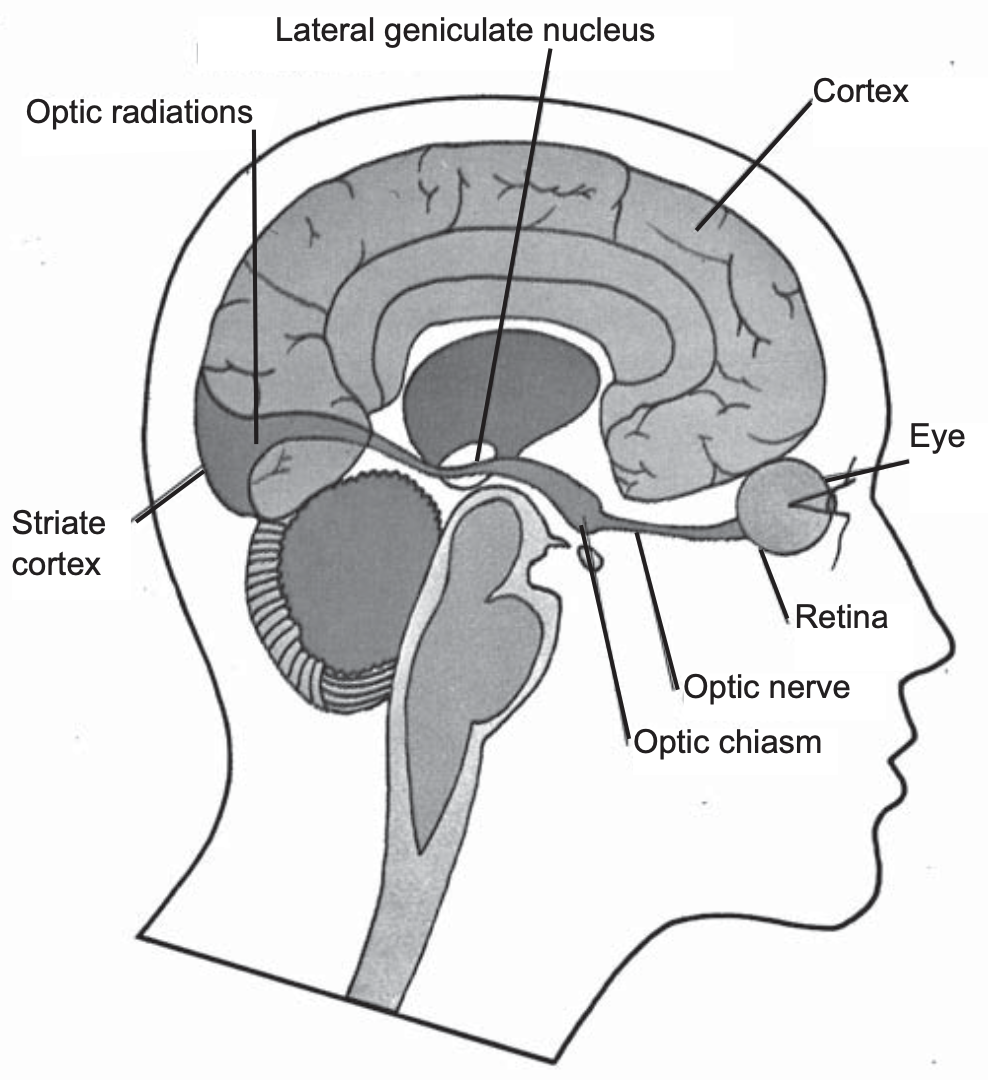
\includegraphics[width=0.4\textwidth]{Figs/brain}
\caption{\textbf{Diagrammatic section through the head} \\ This shows principal features of the major visual pathway that links the eyes to the cortex.}
\label{fig:brain}
\end{figure}
\end{center}
	
	Visual processing in the brain is a complex and multi-stage process involving several key regions and mechanisms. Initially, photons are captured by photoreceptive cells in the retina. This raw visual data undergoes an initial compression by ganglion cells, reducing its volume by a factor of approximately 150 times. The compressed data is then transmitted to two critical subcortical structures: the Lateral Geniculate Nucleus (LGN) of the thalamus and the superior colliculus (SC) of the midbrain.

Despite the LGN receiving only about 10\% of the total visual information, this still represents a significant volume, surpassing the entire volume of fibers that constitute the auditory tract. The LGN and SC, rooted in the oldest parts of the brain, serve as crucial processing stations before the information ascends to higher cortical areas.

Once the visual data reaches the thalamus, it is further relayed to the primary visual cortex (PVC), located in the occipital lobe at the back of the brain. By the time the information arrives at the PVC, it has not only been significantly compressed but also processed by four distinct types of neurons, ensuring that the visual information is highly refined and organized for higher-level processing.


The visual cortex comprises more than 30 distinct sections, each specializing in different aspects of visual processing. Most studies on the visual cortex have been conducted on monkeys, leading to a relative scarcity of direct evidence about human visual neural pathways compared to those of animals. Despite noticeable anatomical differences between humans and other animals, functional similarities are significant. For example, the V5 area in macaque monkeys, which contains neurons that activate when an object enters the visual field, has also been identified in humans.

Visual perception is produced by cells that fire in a hierarchical manner, encoding features from simple to complex. A cell that activates in response to a complex object is referred to as a gnostic cell. Memory plays a crucial role in this process, as visual perception involves matching incoming stimuli with pre-coded objects in the brain. However, the mechanisms by which the brain encodes new objects remain largely unknown. One supported theory is ensemble firing, which suggests that visual perception results from the collective activity of many cells rather than the exclusive action of gnostic cells. This firing is more efficient when objects are quickly recognized or matched with existing memories.

It is important to note that the superior colliculus (SC) contains sites with cells that respond to multiple sensory inputs. The SC plays a significant role in controlling and orienting movement, suggesting that brain evolution has favored the integration of multiple senses to guide reflexive actions and behaviors crucial for survival. Studies show that the combined response from multiple stimuli in the SC is greater than the sum of responses from each individual stimulus, a process known as multisensory integration.

	\hfill
	
	\subsubsection{What and the Where Visual Pathways}
	
	The what pathway is represented by a ventral cortical stream of fibers which respond to a large field of view. The function of this pathway is to identify the object. Shape, color, and motion are critical clues in that process. The where pathway follows a dorsal cortical stream projecting on to the parietal lobe which is also responsible for the management of our attention. The where pathway responds to a much more limited field of view than the what pathway. In effect, the ventral pathway specializes in recognizing while the dorsal pathway manages what comes next in the form of an action or a plan. It can be said that we have two visual perception systems at play in any given situation, one to help us label the stimuli and another to guide our interaction with it or with the context it creates.

While recent imaging studies do show that there are specific neural pathways producing our visual percepts, such experiments are difficult to conduct. That is why it is important we now review the dominant cognitive theories developed on visual perceptions over the last century. We will then revisit the neuroscientific evidence produced in the last decade to propose an integrative theory of visual perception.


\begin{figure}[H]
\centering
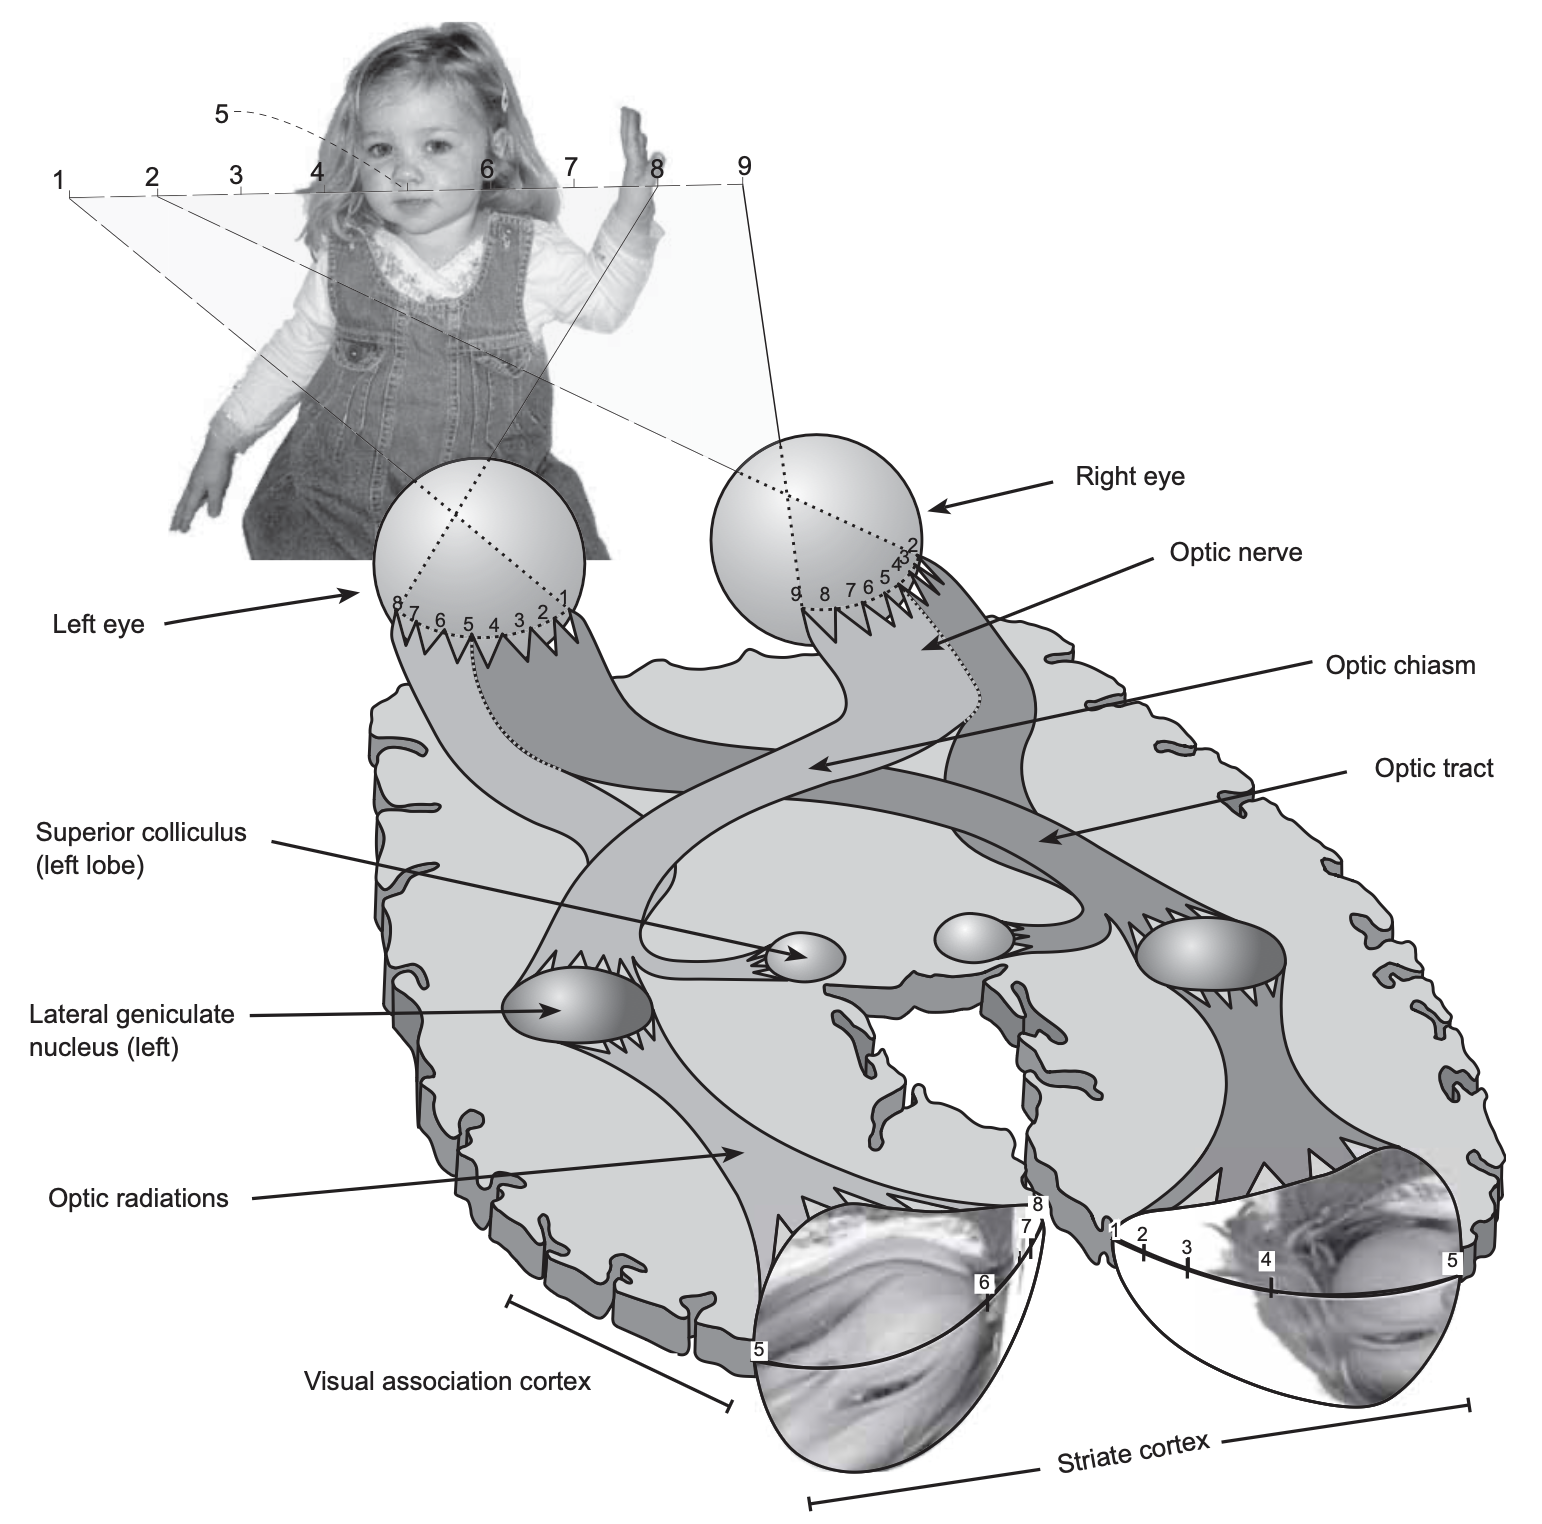
\includegraphics[width=0.8\textwidth]{Figs/pathway}
\caption{\textbf{Schematic illustration of two important visual pathways} \\ One pathway goes from the eyes to the striate cortex and one from the eyes to each superior colliculus. The distortion in the brain mapping in the striate cortex reflects the emphasis given to analysing the central region of the retinal image, so much so that the tiny representation of the child’s hand can hardly be seen in this figure.}
\label{fig:pathway}
\end{figure}
\end{center}



	\subsection{Intra-Layer Neuronal Mechanisms}
	
	\subsubsection{Lateral Inhibition}
	
	Lateral inhibition is the phenomenon in which a neuron's response to a stimulus is inhibited by the excitation of a neighboring neuron. Lateral inhibition has been experimentally observed in the retina and the LGN of organisms. Lateral inhibition makes neurons more sensitive to spatially varying of stimulus than to spatially uniform stimulus. This is because a neuron getting stimulated by a spatially uniform stimulus is also inhibited by its surrounding neurons, thus suppressing its response. On the other hand, a neuron subjected to a spatially varying stimulus is less inhibited by its neighbors that are not excited, thus producing stronger response. Therefore in the case of visual neurons, lateral inhibition makes them more sensitive to edges on the scene. Although usually described for visual neurons, lateral inhibition is also found in other sensory systems, such as auditory and olfactory neurons. The total region, to which a particular neuron is sensitive to, is called the receptive field of the neuron.

The goal of this experiment is to determine if Lateral Inhibition can enhance the neural differentiation process, leading to a clearer and more distinct pattern recognition capability in the output neurons.




\subsubsection[KWTA]{KWTA\footnote{K Winners Take All}}
	
K-Winners-Take-All (KWTA) spiking neural networks are designed to select K elements from a total of N elements based on their activity levels, where the K selected elements have higher activation values than the remaining $N-K$ elements. When $𝐾=1$, the KWTA network functions as a Winner-Take-All (WTA) network, which identifies the neuron with the maximum activation.

Selecting the $K$ largest elements from a set of $N$ real numbers is crucial in decision-making, pattern recognition, associative memories, and competitive learning networks. Such tasks are common in classification problems and are essential for developing spiking neural network classifiers, as well as for solving pattern recognition and classification issues.

	
	The implementation concept of KWTA is that if  $ v \ge threshold$, then $v$ is set to $v_{reset}$, and all other spiked neurons are inhibited.
	
	
	
	\subsubsection{Homeostasis}
	
The human body consists of trillions of cells working together to maintain the organism's overall health and functionality. Despite their diverse functions, these cells share similar metabolic requirements. To ensure the well-being of both individual cells and the entire organism, it is crucial to maintain a constant internal environment that provides necessary elements such as oxygen, glucose, mineral ions, and waste removal. The various processes that regulate this internal environment are collectively known as homeostasis.

Homeostasis refers to the stability, balance, or equilibrium of the body's internal environment. It involves the body's continuous efforts to maintain a constant and balanced state through persistent monitoring and adjustments in response to changing conditions. This process, known as homeostatic regulation, comprises three key components: the receptor, the control center, and the effector.

\begin{itemize}
\item The Receptor: Detects changes in the environment.
\item The Control Center: Receives and processes information from the receptor.
\item The Effector: Responds to the control center's commands by either opposing or enhancing the stimulus.
\end{itemize}

These components work together to restore and maintain homeostasis. For example, in regulating body temperature, temperature receptors in the skin send information to the brain (the control center), which then signals effectors such as blood vessels and sweat glands in the skin. Due to the constant changes in both the internal and external environment, the body must continuously make adjustments to stay at or near a specific value, known as the set point.

\begin{figure}[H]
\centering
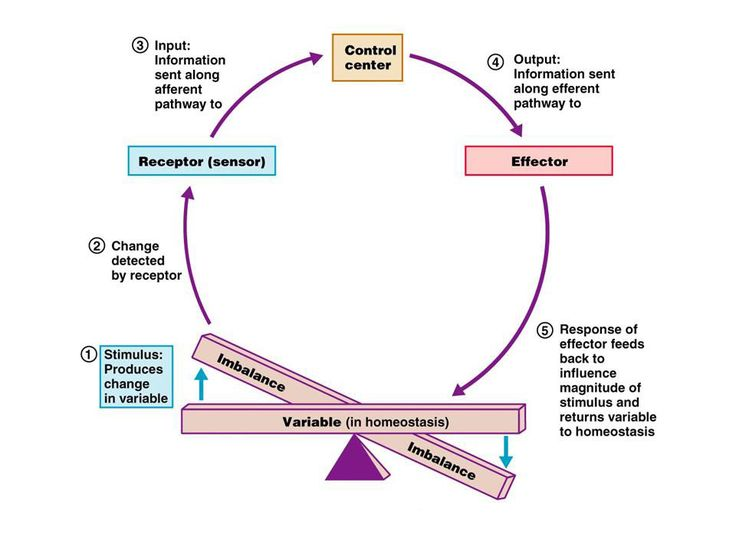
\includegraphics[width=0.7\textwidth]{Figs/h.jpg}
\caption{Homeostasis: positive/ negative feedback mechanisms example}
\label{fig:ce1}
\end{figure}
\end{center}

The primary goal of homeostasis is to maintain equilibrium around the set point. While there are normal fluctuations from this set point, the body's systems strive to return to it. When a stimulus causes a change in the internal or external environment, a receptor detects this change, and the system responds by adjusting the parameter back towards the set point. For instance, if the body becomes too warm, mechanisms are activated to cool it down. Similarly, if blood glucose levels rise after a meal, the body adjusts by moving glucose into tissues that need it or storing it for later use, thereby lowering the blood glucose level.

By continuously regulating these processes, homeostasis ensures the stability necessary for the cells and the organism to function optimally.



\subsection{Neural Coding}

\subsubsection{Time To First Spike} \label{TTFS}

In the TTFS (Time-to-First-Spike) encoding method, we focus on the timing of the neuron's first spike. Specifically, we record and encode the interval from the moment the input is presented to the neuron until it fires. This interval is considered to contain the relevant information. A schematic representation of this process can be seen in Figure \ref{Fig:ttfs}
}.



\begin{figure}[H]
\centering
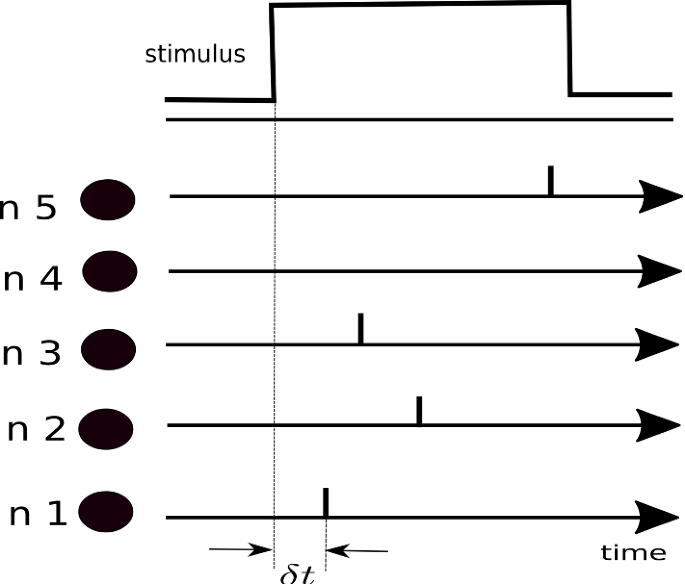
\includegraphics[width=4.5cm]{Figs/ttfs.png}
\caption{\lr{Time To First Spike}}
\label{Fig:ttfs}
\end{figure}
\end{center}

To implement this method, we normalize the inputs to a range, such as 0 to 1, and use a parameter 
$T$ . We divide the 0 to 1 range into $T$ equal intervals. The neuron will spike at the time corresponding to the interval in which the input falls. This process is illustrated in Figure \ref{Fig:int}.

\begin{figure}[H]
\centering
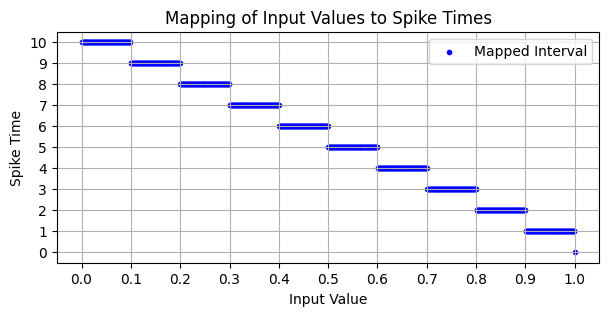
\includegraphics[width=7cm]{Figs/interval.png}
\caption{Simulation of TTFS}
\label{Fig:int}
\end{figure}
\end{center}

Now, using the implemented encoding, we will encode four different images both in their original and compressed forms. The results and the raster plot can be seen in Figure \ref{Fig:ttfs_res}.

\begin{figure}[H]
\centering
  \begin{subfigure}[b]{0.45\textwidth}
    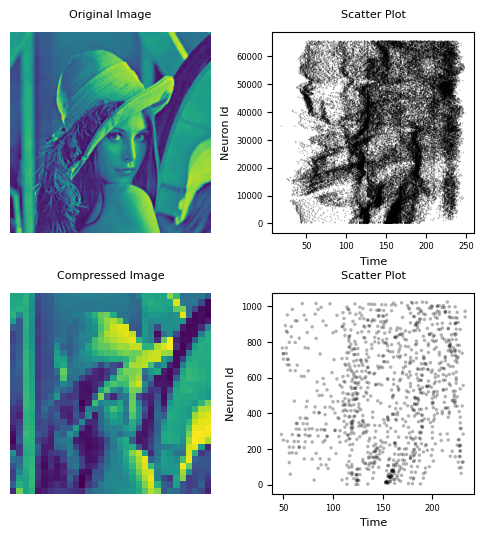
\includegraphics[width=\textwidth]{Figs/ttfs_lena.png}
  \end{subfigure}
  \hfill
  \begin{subfigure}[b]{0.45\textwidth}
    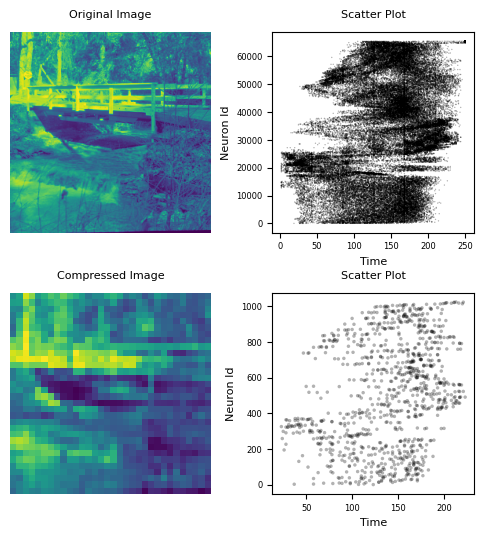
\includegraphics[width=\textwidth]{Figs/ttfs_bridge.png}
  \end{subfigure}
  \caption{Raster plot of spikes that generated using the TTFS encoding method}
  \label{Fig:ttfs_res}
\end{figure}
\end{center}

\subsubsection{Poisson Coding} \label{Poisson}

In this encoding method, the time between generated spikes is obtained using a Poisson distribution. The shape of the Poisson distribution can be seen in Figure \ref{Fig:p-d}. As shown, this distribution includes a parameter $\lambda$, which we set to $0.09$ in our experiment. Finally, similar to the previous sections, the input was provided over a duration of $T = 60ms$, and the result can be seen in Figure \ref{Fig:pc_res}.


\begin{figure}[H]
\centering
  \begin{subfigure}[b]{0.45\textwidth}
    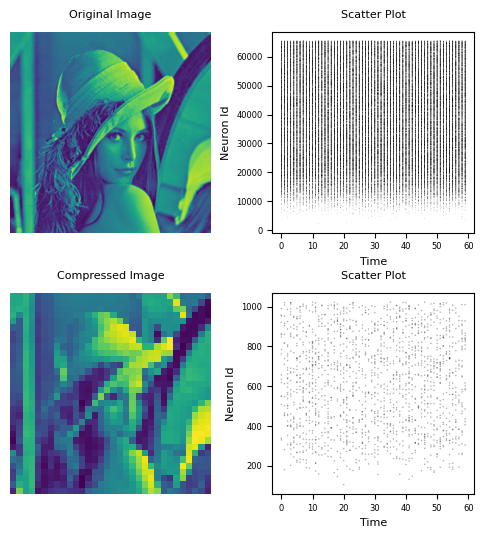
\includegraphics[width=\textwidth]{Figs/p_lena.png}
  \end{subfigure}
  \hfill
  \begin{subfigure}[b]{0.45\textwidth}
    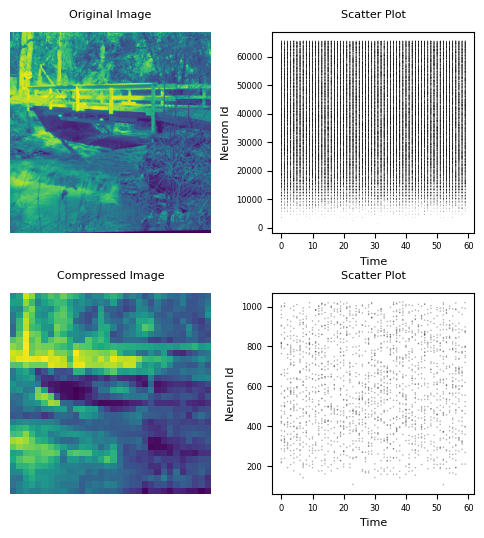
\includegraphics[width=\textwidth]{Figs/p_bridge.png}
  \end{subfigure}
  \caption{Raster plot of spikes that generated using the Poison encoding method}
  \label{Fig:pc_res}
\end{figure}
\end{center}


\begin{figure}[H]
\centering
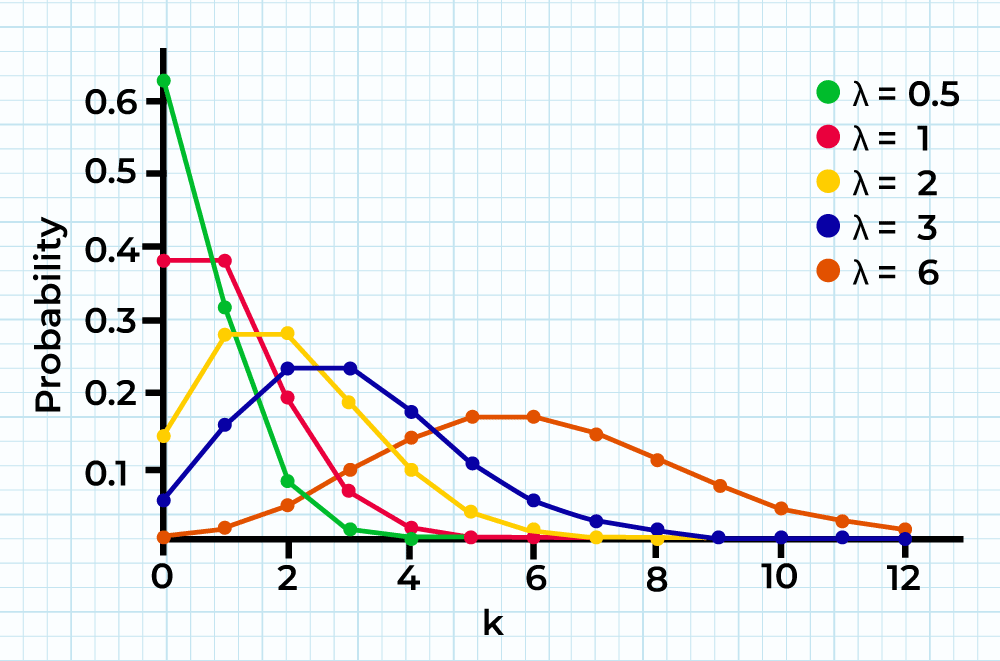
\includegraphics[width=9cm]{Figs/p-d.png}
\caption{Poisson Distribution}
\label{Fig:p-d}
\end{figure}
\end{center}

Here, in the Poisson distribution, the parameter $\lambda$ actually represents the rate or intensity of events. Increasing $\lambda$ results in more events occurring, because a higher $\lambda$ increases the likelihood of an event happening. For instance, in the context of a bird image, we test this experiment with various values of $\lambda$ and visualize the results in Figure \ref{Fig:lambda_res}.


\begin{figure}[H]
\centering
  \begin{subfigure}[b]{0.35\textwidth}
    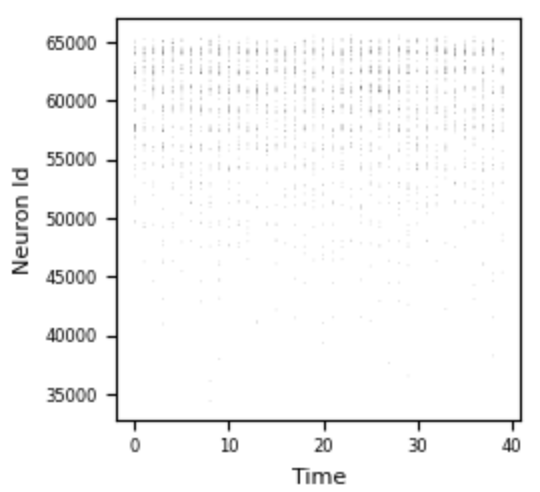
\includegraphics[width=\textwidth]{Figs/1}
    \caption{$\lambda = 0.03$}
  \end{subfigure}
  \hspace*{50}
  \begin{subfigure}[b]{0.35\textwidth}
    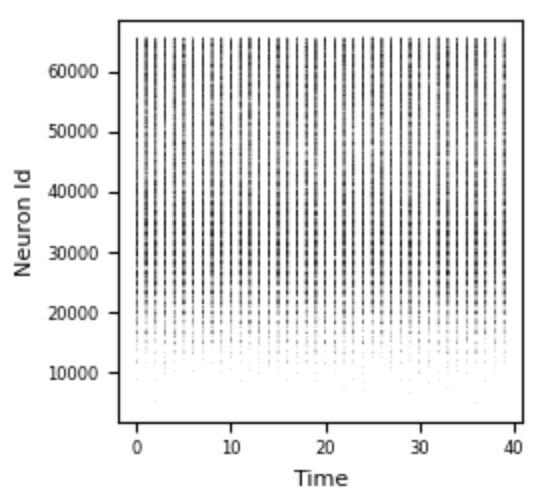
\includegraphics[width=\textwidth]{Figs/2}
    \caption{$\lambda = 0.08$}
  \end{subfigure}
  \\[\smallskipamount]
  \begin{subfigure}[b]{0.35\textwidth}
    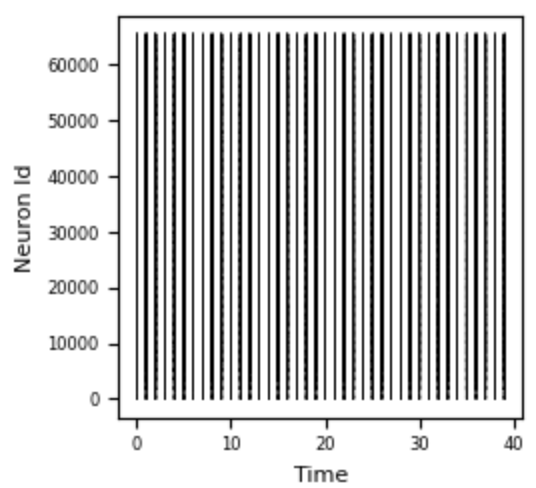
\includegraphics[width=\textwidth]{Figs/3}
    \caption{$\lambda = 0.5$}
  \end{subfigure}
  \hspace*{50}
  \begin{subfigure}[b]{0.35\textwidth}
    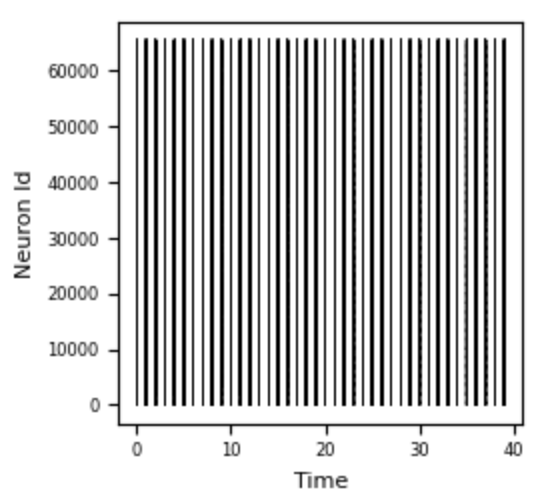
\includegraphics[width=\textwidth]{Figs/4}
    \caption{$\lambda = 1.0$}
  \end{subfigure}
  \caption{The role of $\lambda$ in spike patterns and frequency}
  \label{Fig:lambda_res}
\end{figure}
\end{center}



\subsection{STDP Learning}


	In the Spike-Timing-Dependent Plasticity (STDP) process, if an input spike to a neuron typically occurs just before the neuron’s output spike, the synaptic connection for that input is strengthened. Conversely, if an input spike generally occurs just after an output spike, the synaptic connection is weakened. This timing-dependent adjustment is the essence of "spike-timing-dependent plasticity." Consequently, inputs likely causing the post-synaptic neuron's excitation become more influential, while inputs that are unlikely to cause the excitation become less influential. Over time, this process refines the network by reinforcing a subset of connections while diminishing the impact of others to nearly zero. Since a neuron generates an output spike when many inputs arrive within a short time frame, the remaining subset of inputs tends to be those that are temporally correlated. Additionally, inputs that consistently precede the output spike and indicate early correlation become the primary inputs to the neuron, effectively optimizing the network for detecting and responding to relevant patterns.

	If we have two electrodes placed within the neuronal membrane, and we use one electrode to stimulate the neuron and the other to measure the neuron’s response, we can observe that if the previous neuron is activated and then the next connected neuron is activated shortly afterward, the synaptic strength between these two neurons increases. This indicates that the change in synaptic weight can be a function of the time difference  $ t_j^f - t_i^f $.
	
	
	

\begin{figure}[H]
\centering
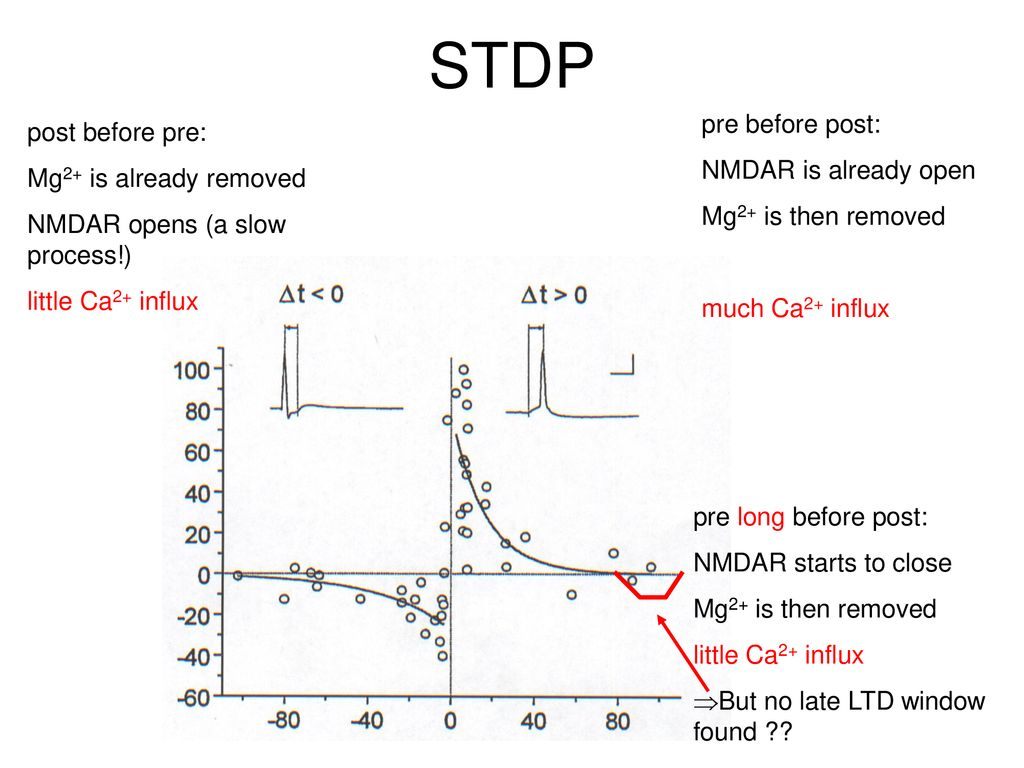
\includegraphics[width=13cm]{Figs/STDP.jpg}
\caption{STDP Leaning Process}
\label{Fig:p-d}
\end{figure}
\end{center}

LTP is the process by which synaptic strength is increased. It occurs when the presynaptic neuron fires just before the postsynaptic neuron. The closer in time these spikes occur, the stronger the synaptic connection becomes. The rationale behind LTP is that if a presynaptic neuron consistently helps to trigger a postsynaptic spike, it should be rewarded by strengthening the connection, making it easier to trigger future spikes. This process reinforces pathways that are frequently used, thereby promoting learning and memory formation.


LTD is the process by which synaptic strength is decreased. It occurs when the presynaptic neuron fires just after the postsynaptic neuron. The further apart these spikes occur, the weaker the synaptic connection becomes. LTD ensures that connections which do not contribute effectively to the postsynaptic activity are weakened. This pruning of less useful synapses is crucial for maintaining the efficiency of the neural network, preventing over-excitation, and ensuring that only the most relevant and effective synaptic pathways are strengthened.



In summary, the STDP learning process can be mathematically simulated using the following equation:

 $$  \frac{dw_{ij}}{dt} = -A_-(w_{ij})y_i(t)\Sigma_f \delta(t-t_j^f) + A_+(w_{ij})x_j(t)\Sigma_f \delta(t-t_i^f)$$
	
	
\section{Methodology}


\subsection{DoG Filter}

	\subsubsection{Retinal Receptive Fields}
	
	The receptive field refers to the specific region of a cell that responds to external stimuli. In the visual system, receptive fields are two-dimensional spaces sensitive to light intensity. The retina, a thin layer of tissue in the eye composed of photoreceptor cells, plays a crucial role in detecting and transmitting visual information to the brain's primary visual cortex via the optic nerve.

In the retina, receptive fields are typically circular and composed of two distinct sub-regions: the center and the surround. These sub-regions exhibit antagonistic preferences for brightness and darkness, categorizing receptive fields into two types: on-center off-surround and off-center on-surround. On-center sub-regions are most responsive to increased light intensity, whereas off-center sub-regions prefer dimmer conditions. This contrast in preferences leads to opposing behaviors between on-center and off-center receptive fields.
	
\begin{figure}[H]
\centering
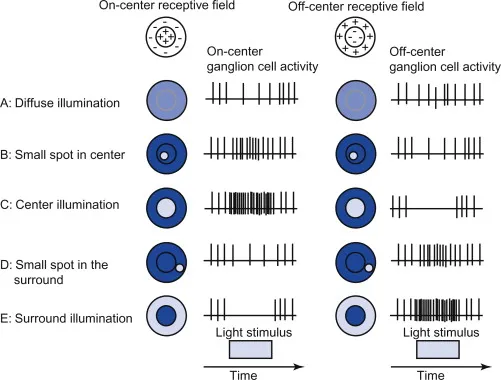
\includegraphics[width=10cm]{Figs/dog.png}
\caption{Functionality of retinal receptive fields}
\label{Fig:dog-filter}
\end{figure}
\end{center}
	
	The left column illustrates the spiking pattern of on-center receptive fields when exposed to different types of stimuli, while the right column details off-center receptive fields. I won't delve into explaining the diagram here, as it can be easily interpreted. Instead, let's focus on these two types of receptive fields on a broader scale.

Imagine a layer of photoreceptor cells with on-center receptive fields responding to a stimulus. Suppose there's an edge dividing a brighter section from a darker one in this stimulus. Given that on-center receptive fields respond most strongly to high intensities, photoreceptor cells with their centers on the bright side of the edge will fire most, while those in the surrounding darker section will fire minimally. Similarly, cells on the bright side of each edge will fire, enhancing the output at a larger scale to reflect the input stimulus with the bright side of each edge accentuated. The opposite response can be expected from a layer of off-center photoreceptor cells.

	\subsubsection{Mathematical Definition}
	
	In the field of image processing, numerous edge detection kernels are widely used today, many of which are convolution matrices designed to enhance edges without explicitly separating outputs related to on and off receptive fields. However, among these kernels, the Difference of Gaussian (DoG) has been notable for its ability to mimic the natural behavior of retinal receptive fields.

The DoG kernel is derived from the difference between two 2-dimensional Gaussian functions with different standard deviation values. Before discussing the results, let's delve into the mathematical foundation of this process.

\hfill
\\


$$ f_1(x, y) = \frac{1}{2\pi\sigma_1^2} exp(-\frac{1}{2\pi\sigma_1^2} (x^2 + y ^2))  $$

$$ f_2(x, y) = \frac{1}{2\pi\sigma_2^2} exp(-\frac{1}{2\pi\sigma_2^2} (x^2 + y ^2))  $$

$$ suppose \; \sigma_1 < \sigma_2 $$

$$ g_1(x,y) = f_1(x,y) - f_2(x, y) \qquad g_2(x, y) = f_2(x, y) - f_1(x, y)$$

\hfill
\\

In above figure, f1 and f2 are 2-dimensional Gaussian functions with $\sigma_1 < \sigma_2$ . And $g_1$ and $g_2$ be differences of Gaussian kernel functions. Following plot includes 3-dimensional and 2-dimensional (top down) views of those functions for your better understanding.

\begin{figure}[H]
\centering
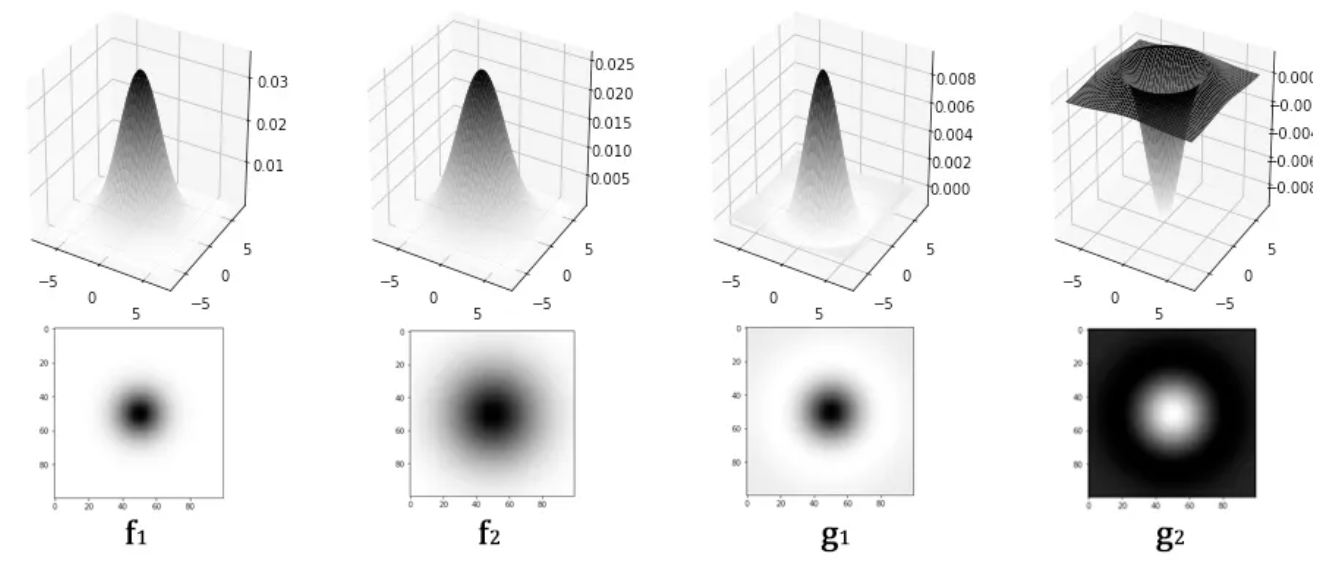
\includegraphics[width=1.0\textwidth]{Figs/top-down}
\caption{3-dimensional and top-down views of Gaussian functions and DoG functions}
\label{fig:top-down}
\end{figure}
\end{center}

We can utilize $g_1$ to simulate on-center off-surround retinal receptive fields and $g_2$ as the kernel for off-center on-surround retinal receptive fields.
	
	\subsubsection{Experiment Results}
	
	We have developed two Difference of Gaussian (DoG) filter kernels of size 10, As I mentioned earlier we use $g_1$ for on-center off-surround and $g_2$
for off-center on-surround, with parameters $\sigma_1 = 1$ and $\sigma_2 = 1.5$. You can view the filters in Figure \ref{Fig:dogkf1}.
	
\begin{figure}[H]
\centering
	\begin{subfigure}[b]{0.22\textwidth}
    
\includegraphics[width=\textwidth]{Figs/kf2.png}
    \caption{on-center off-surround, $g_1$}
  \end{subfigure}
  \hspace{80}
  \begin{subfigure}[b]{0.22\textwidth}
    
\includegraphics[width=\textwidth]{Figs/dogkf1.png}
    \caption{off-center on-surround, $g_2$}
  \end{subfigure}
  \caption{DoG kernels with parameters $\sigma_1 = 1$ and $\sigma_2 = 1.5$}
  \label{Fig:dogkf1}
\end{figure}
\end{center}

Now, we apply these kernels to a grayscale image through convolution.

\begin{figure}[H]
\centering
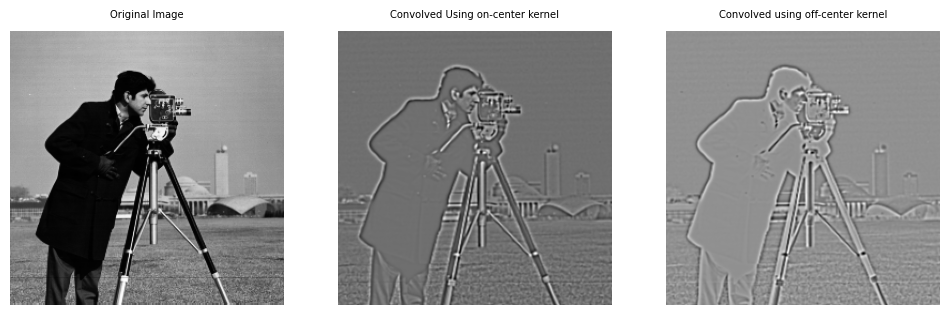
\includegraphics[width=0.9\textwidth]{Figs/cdog.png}
\caption{Effect of DoG kernel on an input stimulus}
\label{fig:cdog}
\end{figure}
\end{center}

We can see inner margins of edges are enhanced while outer margins of edges are weakened after convolving with $g_1$ kernel, which is he behavior of on-center retinal receptive fields. Also, in the right most figure, outer margins of edges are enhanced, and inner margins are weakened after convolving with $g_2$ kernel as we can expect from off-center receptive fields.

Contrast of the enhancement (edge detection) can be optimized using tuning the standard deviation values.

	\subsubsection{Parameter Analysis}
	
	As mentioned earlier, the Difference of Gaussian (DoG) filter is defined by two important parameters: 
$\sigma_1$ and $\sigma_2$. The selection of these parameters significantly influences the characteristics and effectiveness of the filter, particularly when modeling simple cells in V1.

For a clearer visualization of the formula, we set $\sigma_1 = 1$ and vary $\sigma_2$. We plot the Gaussian distributions and their differences. As shown in the results in Figure \ref{Fig:dogparam}, increasing $\sigma_2$ makes our Difference of Gaussians (DoG) resemble the initial Gaussian more closely and This means more sensitivity to broader spatial structures that enables effectively capture edges and transitions. It enhances the contrast between central and surrounding regions, thereby making edges more distinct.


\begin{figure}[H]
\centering
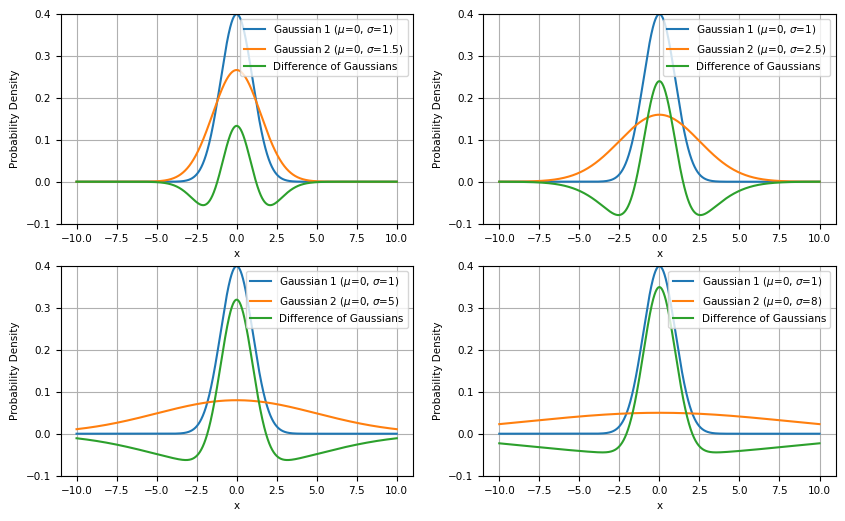
\includegraphics[width=0.85\textwidth]{Figs/dogparam.png}
\caption{Difference of Gaussian with different $\sigma_2$}
\label{fig:dogparam}
\end{figure}
\end{center}
	
	Based on the distribution, we create two different kernels with the same $\sigma_1$ but different $\sigma_2$, as shown in Figure \ref{Fig:ddof}.
	
	\begin{figure}[H]
\centering
	\begin{subfigure}[b]{0.17\textwidth}
    
\includegraphics[width=\textwidth]{Figs/s11s21.5.png}
    \caption*{$\sigma_2 = 1.5$}
  \end{subfigure}
  \hspace{10}
  \begin{subfigure}[b]{0.17\textwidth}
    
\includegraphics[width=\textwidth]{Figs/s11s21.52.png}
    \caption*{$\sigma_2 = 1.5$}
  \end{subfigure}
  \hspace{10}
  \begin{subfigure}[b]{0.17\textwidth}
    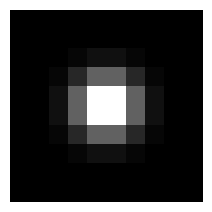
\includegraphics[width=\textwidth]{Figs/s11s28.png}
    \caption*{$\sigma_2 = 8$}
  \end{subfigure}
  \hspace{10}
  \begin{subfigure}[b]{0.17\textwidth}
    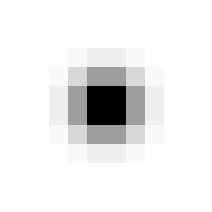
\includegraphics[width=\textwidth]{Figs/s11s282.png}
    \caption*{$\sigma_2 = 8$}
  \end{subfigure}
  \caption{DoG kernels with parameters $\sigma_1 = 1$ and different $\sigma_2$}
  \label{Fig:ddof}
\end{figure}
\end{center}

	Now, we convolve these kernels with the same input image and compare their results.	
	
\begin{figure}[H]
\centering
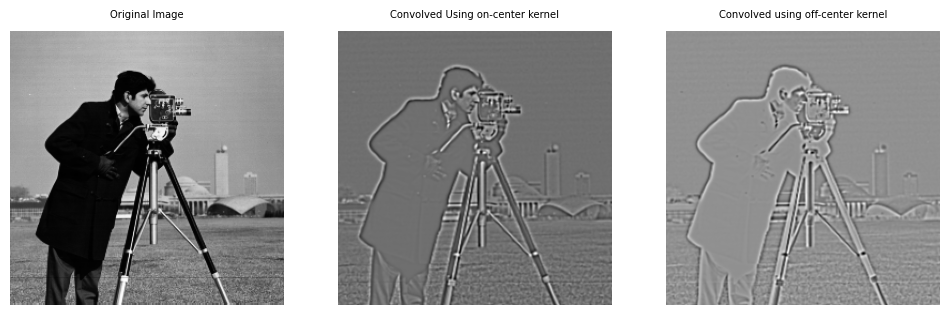
\includegraphics[width=0.9\textwidth]{Figs/cdog.png}
\caption{Effect of DoG kernel with $\sigma_2 = 1.5$ on an input stimulus}
\label{fig:param1}
\end{figure}
\end{center}

\begin{figure}[H]
\centering
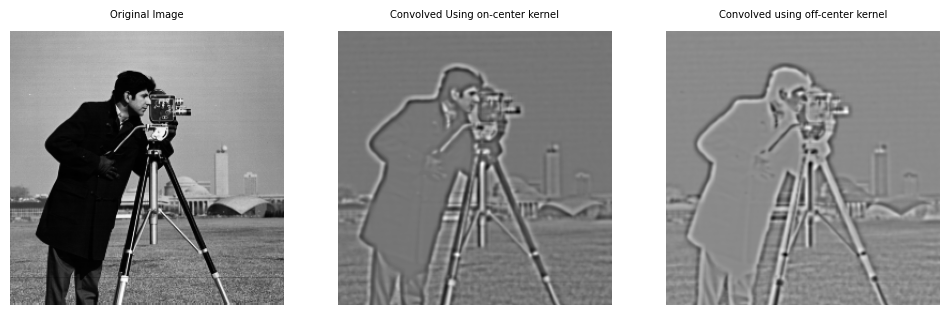
\includegraphics[width=0.9\textwidth]{Figs/convolved2.png}
\caption{Effect of DoG kernel with $\sigma_2 = 8$ on an input stimulus}
\label{fig:param2}
\end{figure}
\end{center}
	
	In conclusion, as depicted in Figure \ref{fig:param1} and Figure \ref{fig:param2}, increasing the differences between $\sigma_1$ and $\sigma_2$ in the Difference of Gaussian (DoG) filter enhances its sensitivity to broader spatial structures. This adjustment allows the filter to effectively capture edges and transitions, enhancing the contrast between the center and surround regions. The broader Gaussian smooths out noise, focusing more on significant changes in the image and making edges more pronounced. Consequently, the filter detects larger-scale features and low-frequency components, thereby capturing broader patterns and significant structures in the image, resulting in a more structured output.

Conversely, when $\sigma_1$ and $\sigma_2$ are closely related, the DoG filter behaves similarly to a single Gaussian filter. In such cases, the filter's response primarily highlights very fine details and small-scale features. However, it may not effectively suppress background noise, leading to less pronounced edge detection.


	\subsubsection{Time To First Spike Coding}

Initially, I created a Difference of Gaussian (DoG) filter with parameters $\sigma_1 = 1$ and $\sigma_2 = 1.5$, as illustrated in Figure \ref{Fig:dogkf1}. This filter was then convolved with the input grayscale image to enhance its edges and transitions.

Next, I prepared two versions of the processed image: the original convolved image and a compressed version obtained through average pooling. This compression step reduces the image resolution while retaining its essential features, aiding in efficient processing.

Both the original and compressed images were subsequently fed into the TTFS encoder, as detailed in section \textbf{\ref{TTFS}}. The TTFS encoder is designed to simulate the temporal dynamics of neuronal responses, converting the processed images into a format suitable for further analysis or classification tasks.

The results, presented below, demonstrate the encoder's ability to effectively process and encode the visual information from the convolved and pooled images. The enhanced edge detection, achieved through the DoG filtering, significantly contributes to the encoder's performance, enabling it to capture and represent crucial image features accurately. By varying the parameters $\sigma_1$ and $\sigma_2$ , we can fine-tune the filter's sensitivity to different spatial frequencies, thereby optimizing the edge detection process for specific applications.


\begin{figure}[H]
\centering
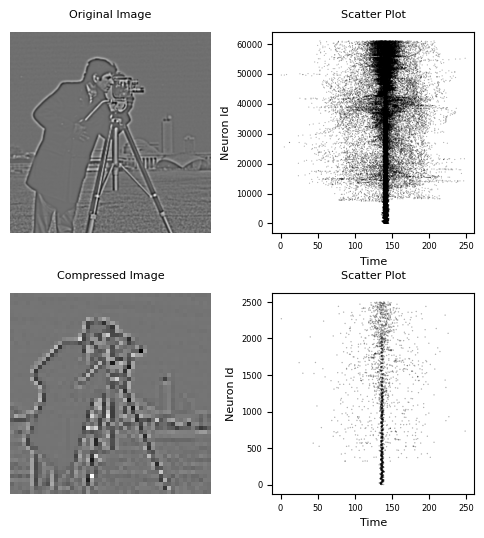
\includegraphics[width=0.47\textwidth]{Figs/ttfsdog.png}
\caption{TTFS Encoding Applied to an Image Convolved with a DoG Kernel}
\label{fig:ttfsdog}
\end{figure}
\end{center}
	
	\subsubsection{Poisson Coding}

	As discussed in the previous section, I initially applied TTFS encoding to the image after it was convolved with a DoG kernel. However, in the final step, I decided to use Poisson Coding instead of TTFS coding. The details of Poisson Coding are described in section \ref{Poisson}.
	
\begin{figure}[H]
\centering
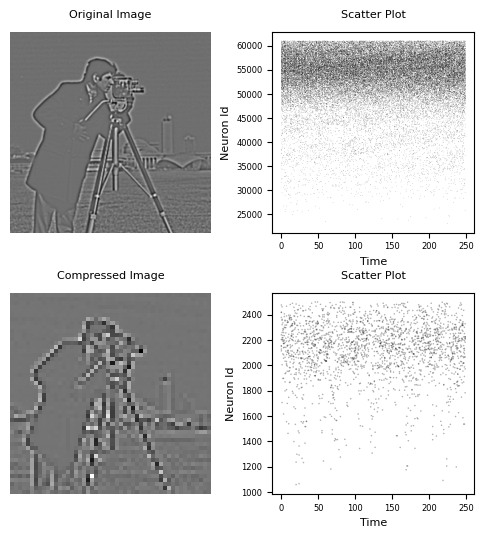
\includegraphics[width=0.47\textwidth]{Figs/poissondog.png}
\caption{Poisson Encoding Applied to an Image Convolved with a DoG Kernel}
\label{fig:poissondog}
\end{figure}
\end{center}	


\subsection{Gabor Filter}

\subsubsection{Primary visual cortex(V1)}

Information from the eye enters the retina, where it is processed by photoreceptor cells and ganglion cells. These ganglion cells detect points of light and transmit this information through the optic nerve to the Lateral Geniculate Nucleus (LGN) of the thalamus. The LGN serves primarily as a relay station, passing the information on to the primary visual cortex (V1) without significant modification. The data entering V1 still maintain a retinotopic organization, meaning the spatial arrangement of the visual field is preserved.

Our understanding of the V1 area is largely based on the groundbreaking experiments conducted by David Hubel and Torsten Wiesel. In their research, they recorded electrical activity from the visual cortex of cats using electrodes. The recorded signals were amplified and connected to a speaker, which emitted sounds whenever neuronal activity was detected. By fixing the cat's head in place and presenting various visual stimuli, they were able to monitor the responses of individual neurons.

\begin{figure}[H]
\centering
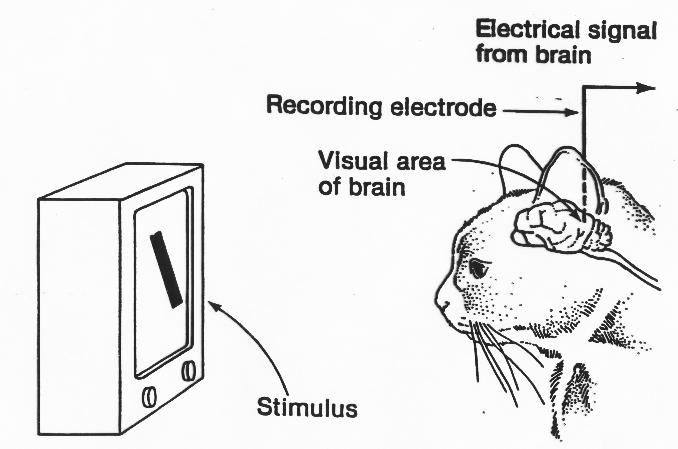
\includegraphics[width=0.42\textwidth]{Figs/hubel.jpg}
\caption{Hubel and Wiesel Experiment}
\label{fig:hubel}
\end{figure}
\end{center}

Their experiments revealed that the V1 area contains neurons tuned to detect lines of specific orientations. Some neurons respond optimally to vertical lines, others to horizontal lines, and still others to various angles in between. Additionally, there are neurons in V1 that are sensitive to the direction of motion. This means that certain neurons will fire when an object moves in a particular direction.

This orientation and motion selectivity of V1 neurons is crucial for processing visual information in two major pathways: the ventral stream and the dorsal stream. The ventral stream, often referred to as the "what" pathway, is involved in object recognition and identification. It processes information about the presence, shape, and color of objects, including the detection of edges and lines. On the other hand, the dorsal stream, known as the "where" pathway, is responsible for spatial awareness and motion detection. It processes information related to the location and movement of objects in the visual field.

Regarding the coverage of all possible angles, V1 does not have neurons for every conceivable angle. Instead, each neuron is most responsive to a particular orientation and also responds, to a lesser degree, to neighboring orientations. By analyzing the collective responses of a population of neurons, the brain can accurately determine the orientation of a perceived line.


\begin{figure}[H]
\centering
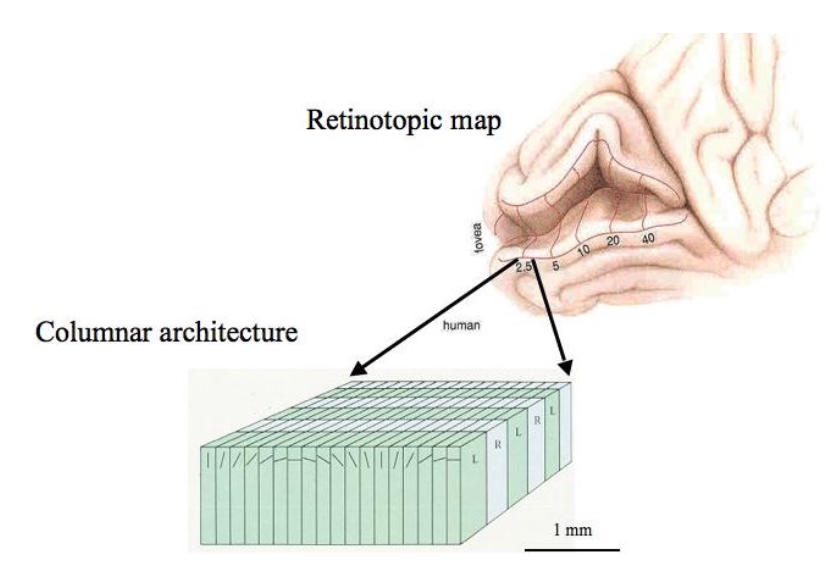
\includegraphics[width=0.42\textwidth]{Figs/colv1}
\caption{\textbf{Columnar architecture of V1} \\ As one moves an electrode vertically through the thickness of cortex, one finds that most neurons have the same selectivity (e.g., the same orientation preference and eye dominance). Ocular dominance columns: As one moves an electrode tangentially through the cortex, one first finds cells that respond to left eye inputs, then binocular (responsive to both/either eye), then right eye, then binocular, then left again, etc. Orientation columns: As one moves the electrode tangentially in the orthogonal direction, one first find cells selective for vertical, then diagonal, then horizontal, etc. A hypercolumn is a chunk of cortex about 1 mm square by 3 mm thickn that contains neurons, all with approximately the same receptive field location, but with all different orientation selectivities, direction selectivities, both (left and right) eye dominances represented.}
\label{fig:colv1}
\end{figure}
\end{center}


In summary, the V1 area plays a fundamental role in the initial processing of visual information, extracting crucial features such as line orientation and motion. This processed information is then relayed to higher visual areas through the ventral and dorsal streams, enabling complex visual perception and interpretation.


\subsubsection{Neurons in V1}

\begin{itemize}

\item[•] \textbf{Simple Cells}

Simple cells are found in the primary visual cortex (V1) and are characterized by their sensitivity to specific orientations of edges or bars of light. They have distinct, structured receptive fields with excitatory and inhibitory regions. The layout of these regions determines their response to specific patterns of light. Simple cells respond maximally when a bar of light of a particular orientation aligns with their receptive field's excitatory region. They are selective for the position, orientation, and sometimes the spatial frequency of the stimulus. We can simulate simple cells with Gabor Filters.

\item[•] \textbf{Complex Cells}

 Complex cells are also located in the primary visual cortex (V1) but have more advanced properties compared to simple cells. Unlike simple cells, complex cells have receptive fields without distinct, fixed excitatory or inhibitory regions. They are more flexible in the spatial arrangement of their receptive fields. Complex cells respond to bars of light of specific orientations, similar to simple cells, but their response is less dependent on the exact position of the stimulus within the receptive field. They can also respond to moving stimuli, making them crucial for detecting motion.

\item[•] \textbf{Hypercomplex Cells}

Hypercomplex cells, also known as end-stopped cells, are a type of neuron found in V1 and beyond, such as in V2 (the secondary visual cortex). These cells have receptive fields that are sensitive to the length of the stimuli in addition to orientation and movement. Hypercomplex cells respond to stimuli of specific orientations and lengths. They are inhibited when the stimulus exceeds a certain length, effectively detecting the ends or corners of objects. This makes them important for identifying shapes and complex features in the visual scene.
\end{itemize}

\subsubsection{How Gabor Filters Simulate Simple Cells in V1}

Simple cells in the primary visual cortex (V1) respond maximally to specific orientations and spatial frequencies of edges or bars of light. Gabor filters are particularly effective at modeling these properties because they can be tuned to detect specific orientations and frequencies, similar to simple cells.


Similarities Between Gabor Filters and Simple Cells are:

\begin{itemize}
\item[•] \textbf{Orientation Selectivity} :  Both Gabor filters and simple cells are sensitive to specific orientations. By adjusting the orientation parameter ($\theta$), a Gabor filter can be made to detect edges at a particular angle, just like simple cells that are tuned to respond to specific edge orientations.

\item[•] \textbf{Spatial Frequency Tuning}: Simple cells respond to specific spatial frequencies of visual stimuli. The wavelength parameter ($\lambda$) in the Gabor filter allows it to be tuned to detect specific spatial frequencies, mirroring the frequency tuning of simple cells.

\item[•] \textbf{Localized Response}: Simple cells have localized receptive fields, meaning they respond to stimuli in a specific region of the visual field. The Gaussian envelope in a Gabor filter ensures that it also has a localized response, capturing features in a specific region of the image.

\item[•] \textbf{Phase Sensitivity}: The phase parameter ($\psi$) in the Gabor filter allows it to be sensitive to different phases of the sinusoidal component. This is similar to how simple cells can respond to different phases of edges or bars of light.

\end{itemize}

\subsubsection{Mathematical Definition}

	A Gabor filter is defined by a sinusoidal wave (a complex exponential) multiplied by a Gaussian function. The 2D Gabor filter can be expressed mathematically as:
	
	$$ g(x, y, \lambda, \theta, \sigma, \psi) = exp(- \frac{x^2+y^2+\psi^2}{2\psi^2}) cos(\frac{2\pi}{\lambda}x) $$
	
	$$ x = x \cos \theta + y \sin \theta $$
	
	$$ y = -x \sin \theta + y \cos \theta $$
	
	The parameters are:
\begin{itemize}

\item[•] $\lambda$ : Wavelength of the sinusoidal factor.

\item[•] $\theta$: Orientation of the normal to the parallel stripes of the Gabor function.

\item[•] $\psi$: Phase offset.

\item[•] $\sigma$: Standard deviation of the Gaussian envelope.

\item[•] $\gamma$: Spatial aspect ratio, which specifies the ellipticity of support of Gabor function.

\end{itemize}


\subsubsection{Experiment Results}

In this section, we generate two Gabor filter kernels with identical parameters except for their orientations. These kernels will demonstrate how Gabor filters can be tuned to detect edges or features in different directions. Here are the resulting filter kernels:

\begin{figure}[H]
\centering
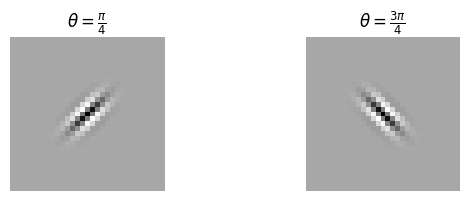
\includegraphics[width=0.45\textwidth]{Figs/gabork.png}
\caption{Gabor kernels with different orientations}
\label{fig:gabork}
\end{figure}
\end{center}

Now, we apply these kernels to a grayscale image through convolution.

\begin{figure}[H]
\centering
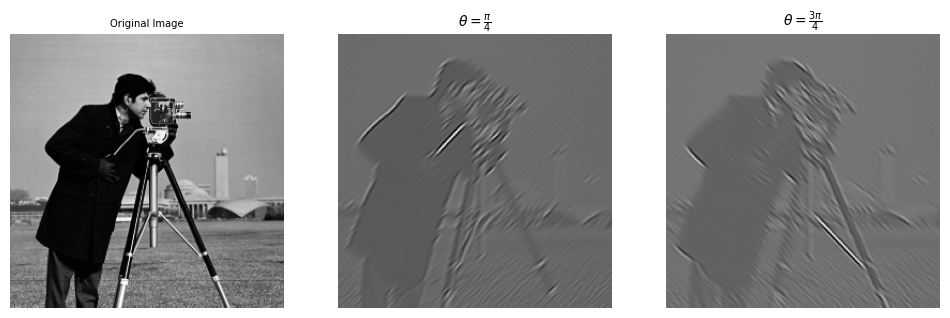
\includegraphics[width=0.85\textwidth]{Figs/gaborres.png}
\caption{Effect of Gabor kernel on an input stimulus}
\label{fig:gaborres}
\end{figure}
\end{center}

\subsubsection{Parameter Analysis}


\paragraph{Spatial wavelength ($\lambda$)}
\hfill

The wavelength ($\lambda$) controls the width of the stripes in the Gabor function. Increasing the wavelength results in wider stripes, while decreasing it produces narrower stripes. By adjusting 
$\lambda}$ to values such as 2.8 and 3.5, while keeping other parameters constant, you will observe that the stripes become progressively thicker.


\begin{figure}[H]
\centering
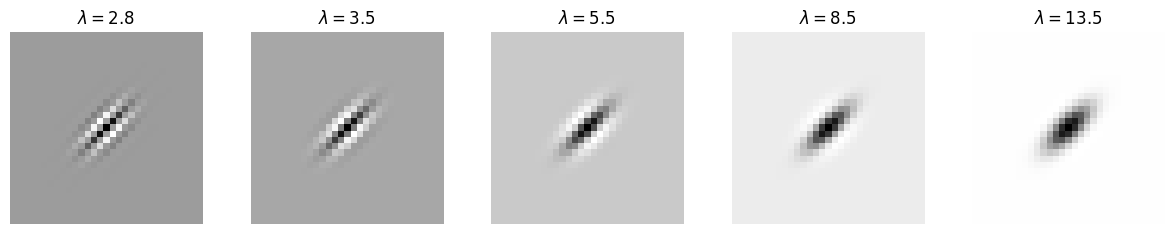
\includegraphics[width=0.95\textwidth]{Figs/lambda.png}
\caption{
Keeping other parameters unchanged ($\theta$ = $\frac{\pi}{4}$, $\gamma$ = 0.5, $\sigma$ = 1.5, $\psi$ = 1), and changing the lambda from 2.8 to 3.5 to 5.5 to 8.5 and 13.5 the Gabor function gets thicker
}
\label{fig:lambda}
\end{figure}
\end{center}

\begin{figure}[H]
\centering
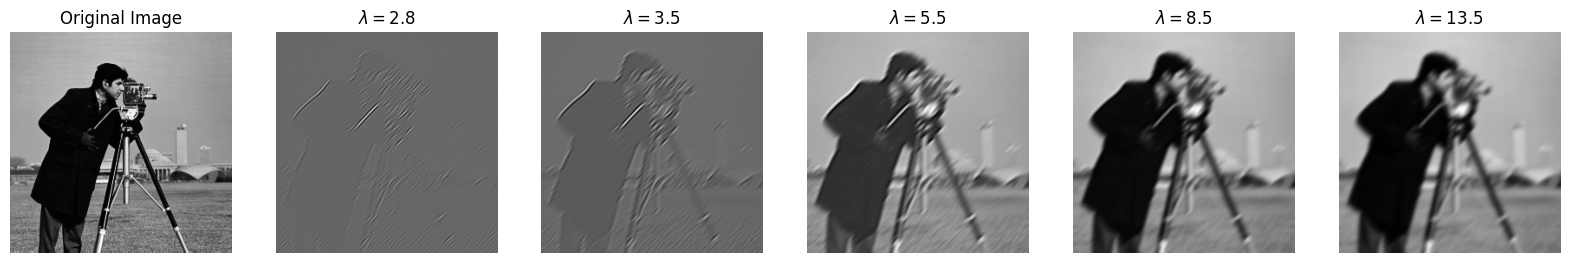
\includegraphics[width=0.95\textwidth]{Figs/labda2.png}
\caption{Effect of Gabor kernel with different spatial wavelength on an input stimulus}
\label{fig:lambda2}
\end{figure}
\end{center}

 Increasing $\lambda$ makes the filter sensitive to low-frequency components of the image. This means that the filter will better capture broad, large-scale features and edges. The filter will respond more to smooth variations in intensity rather than sharp, fine details.


\paragraph{Orientation ($\theta$)} 
\hfill

The angle parameter ($\theta$) determines the filter’s preferred spatial orientation and the direction of motion sensitivity. For example, when $\theta = 0$, the filter responds most strongly to vertical edges moving horizontally to the right. This parameter is specified in degrees and can take values in the range [0, 360).

\begin{figure}[H]
\centering
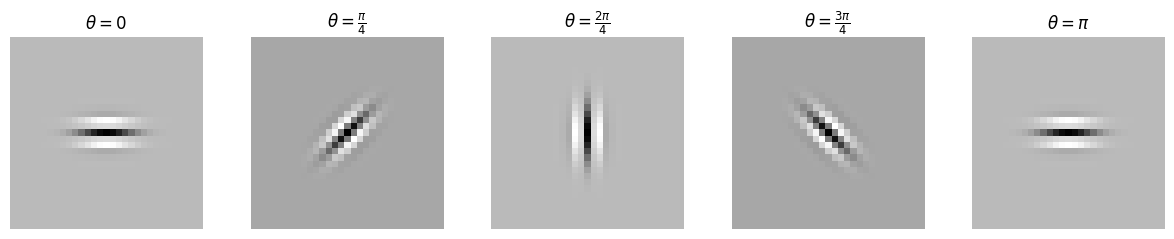
\includegraphics[width=0.95\textwidth]{Figs/theta.png}
\caption{
Keeping other parameters unchanged ($\lambda$ = 3.5, $\gamma$ = 0.5, $\sigma$ = 1.5, $\psi$ = 1), and on changing the theta from 0 to 45 to 90 to 135 and 180 the Gabor function rotates.
}
\label{fig:theta}
\end{figure}
\end{center}

\begin{figure}[H]
\centering
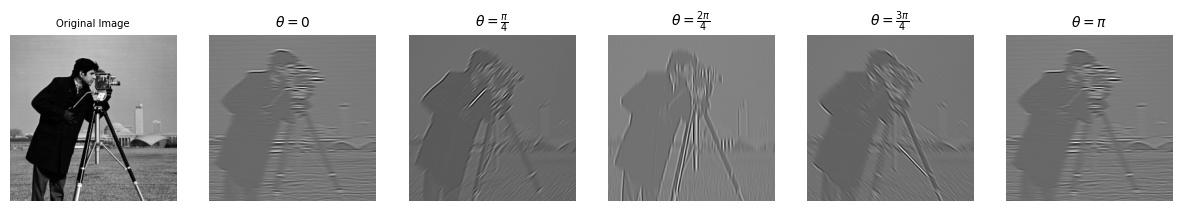
\includegraphics[width=0.95\textwidth]{Figs/theta2.png}
\caption{Effect of Gabor kernel with different orientation on an input stimulus}
\label{fig:theta2}
\end{figure}
\end{center}

Changing the orientation changes the direction of the edges that the filter detects. A filter oriented at 
$\theta = 0$ degrees will detect vertical edges, whereas a filter at $\theta = 90$ degrees will detect horizontal edges. Features in the image that are aligned with the filter’s orientation will be enhanced. For instance, if the filter is oriented at 45 degrees, diagonal edges at 45 degrees will be highlighted.


\paragraph{Spatial aspect ratio ($\gamma$)}
\hfill

The aspect ratio or gamma controls the height of the Gabor function. For a very high aspect ratio the height becomes very small and for a very small gamma value the height becomes quite large. On increasing the value of gamma to 0.5 and 0.75, keeping other parameters unchanged, the height of the Gabor function reduces.

\begin{figure}[H]
\centering
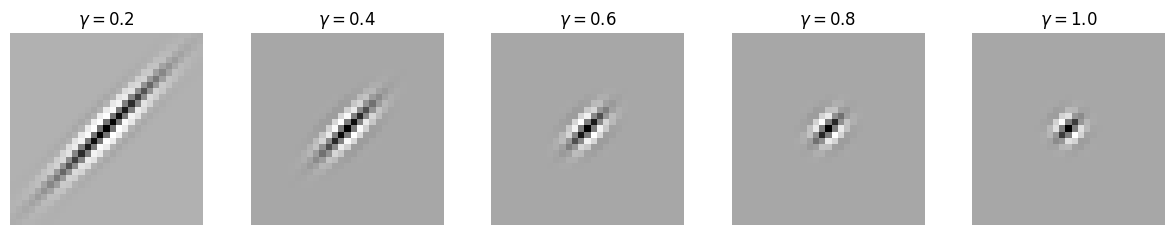
\includegraphics[width=0.95\textwidth]{Figs/gamma.png}
\caption{
Keeping other parameters unchanged ($\lambda$ = 3.5, $\theta$ = $\frac{\pi}{4}$, $\sigma$ = 1.5, $\psi$ = 1), and on changing the gamma from 0.2 to 0.4 to 0.6 to 0.8 and 1, the Gabor function gets shorter.}
\label{fig:gamma}
\end{figure}
\end{center}

\begin{figure}[H]
\centering
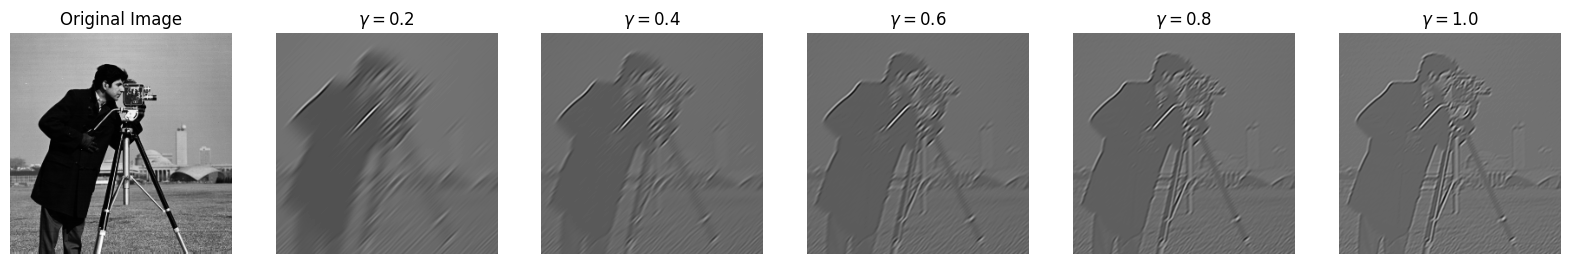
\includegraphics[width=0.95\textwidth]{Figs/gamma2.png}
\caption{Effect of Gabor kernel with different spatial aspect ratio on an input stimulus}
\label{fig:gamma2}
\end{figure}
\end{center}

Increasing $\gamma$ makes the filter more sensitive to features aligned along the y-axis. This means that vertical edges or textures will be more prominently detected on the other hand  the filter becomes less sensitive to features aligned along the x-axis.

\paragraph{Standard deviation ($\sigma$)}
\hfill

The bandwidth or sigma controls the overall size of the Gabor envelope. For larger bandwidth the envelope increase allowing more stripes and with small bandwidth the envelope tightens.On increasing the sigma to 1 and 3, the number of stripes in the Gabor function increases.

\begin{figure}[H]
\centering
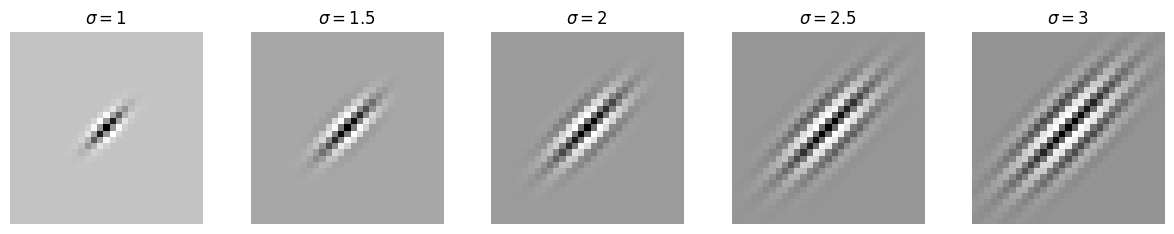
\includegraphics[width=0.95\textwidth]{Figs/sigma.png}
\caption{
Keeping other parameters unchanged ($\lambda$ = 3.5, $\theta$ = $\frac{\pi}{4}$, $\gamma$ = 0.4, $\psi$ = 1), and on changing the sigma from 1 to 1.5 to 2 to 2.5 and 3 the number of stripes in the Gabor function increases.}
\label{fig:sigma}
\end{figure}
\end{center}

\begin{figure}[H]
\centering
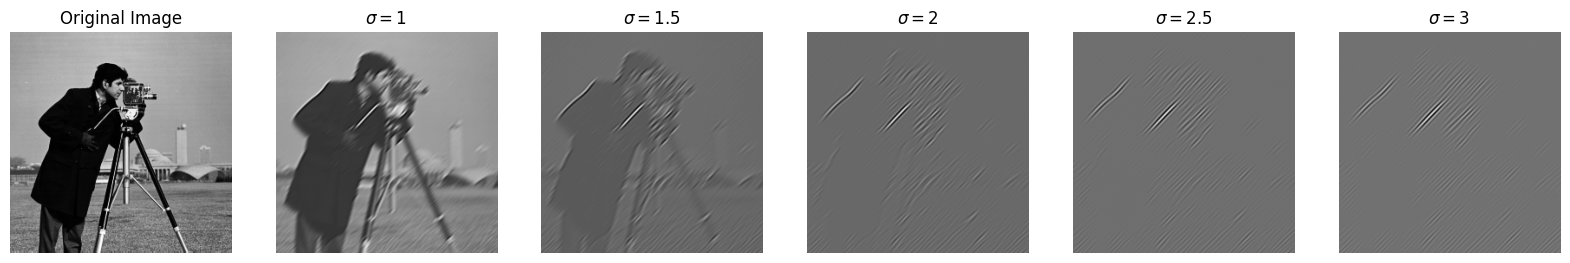
\includegraphics[width=0.95\textwidth]{Figs/sigma2.png}
\caption{Effect of Gabor kernel with different standard deviation on an input stimulus}
\label{fig:sigma2}
\end{figure}
\end{center}

Increasing $\sigma$ results in a wider Gaussian envelope. This makes the filter less sensitive to small-scale details and more sensitive to larger-scale features. A larger $sigma$ leads to a smoothing effect, reducing noise and fine details while emphasizing broader structures.


\subsubsection{Time To First Spike Coding}

Initially, I created a Gabor filter with parameters $\lambda = 3.5$,  $\sigma = 1.5$, $\gamma = 0.5$ and $\theta = \frac{\pi}{4}$, as illustrated in Figure \ref{fig:gabork}. This filter was then convolved with the input grayscale image to enhance its edges and transitions.

Next, I prepared two versions of the processed image: the original convolved image and a compressed version obtained through average pooling. This compression step reduces the image resolution while retaining its essential features, aiding in efficient processing.

Both the original and compressed images were subsequently fed into the TTFS encoder, as detailed in section \textbf{\ref{TTFS}}. The TTFS encoder is designed to simulate the temporal dynamics of neuronal responses, converting the processed images into a format suitable for further analysis or classification tasks.

The results, presented below, demonstrate the encoder's ability to effectively process and encode the visual information from the convolved and pooled images. The enhanced edge detection, achieved through the Gabor filtering, significantly contributes to the encoder's performance, enabling it to capture and represent crucial image features.


\begin{figure}[H]
\centering
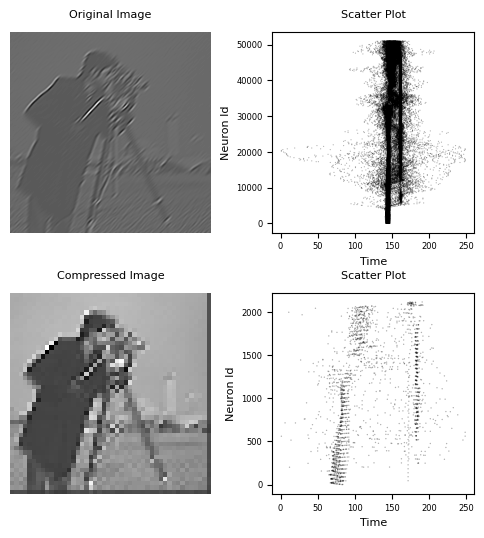
\includegraphics[width=0.47\textwidth]{Figs/gaborttfs.png}
\caption{TTFS Encoding Applied to an Image Convolved with a Gabor Kernel}
\label{fig:gaborttfs}
\end{figure}
\end{center}
	
	\subsubsection{Poisson Coding}

	As discussed in the previous section, I initially applied TTFS encoding to the image after it was convolved with a Gabor kernel. However, in the final step, I decided to use Poisson Coding instead of TTFS coding. The details of Poisson Coding are described in section \ref{Poisson}.
	
\begin{figure}[H]
\centering
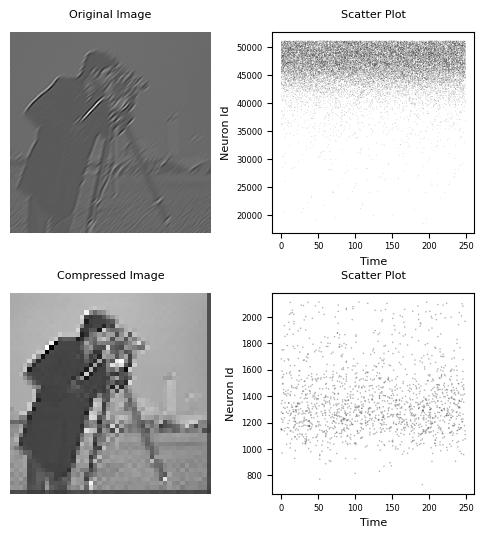
\includegraphics[width=0.47\textwidth]{Figs/poissongabor.png}
\caption{Poisson Encoding Applied to an Image Convolved with a Gabor Kernel}
\label{fig:poissongabor}
\end{figure}
\end{center}	

	
	
	\subsection{Spiking Neural Network}
	
	
\end{document}